\documentclass[conference]{IEEEtran}
\usepackage{natbib}
\usepackage{graphicx}
\usepackage{hyperref}
\graphicspath{{./images/}}

\begin{document}
\title{Update for gazeNet, the end-to-end eye-movement event detection framework with deep neural networks\\
% \thanks{Identify applicable funding agency here. If none, delete this.}
}

\author{\IEEEauthorblockN{1
\textsuperscript{st} Lorenz Falcioni}
\IEEEauthorblockA{
\textit{Faculty of EE and IT} \\
\textit{Ostbayerische Technische Hochschule Regensburg}\\
Regensburg, Germany \\
lorenz2.falcioni@st.oth-regensburg.de}

\and
\IEEEauthorblockN{2
\textsuperscript{nd} Timur Ezer}
\IEEEauthorblockA{
\textit{Laboratory for Safe and Secure Systems (LaS³)} \\
\textit{Ostbayerische Technische Hochschule Regensburg}\\
Regensburg, Germany \\
timur.ezer@oth-regensburg.de}

\and
\IEEEauthorblockN{3
\textsuperscript{rd} Jürgen Mottok}
\IEEEauthorblockA{
\textit{Laboratory for Safe and Secure Systems (LaS³)} \\
\textit{Ostbayerische Technische Hochschule Regensburg}\\
Regensburg, Germany \\
juergen.mottok@oth-regensburg.de}

\and
\IEEEauthorblockN{4
\textsuperscript{rd} Max Mustermann}
\IEEEauthorblockA{
\textit{Laboratory for Safe and Secure Systems (LaS³)} \\
\textit{Ostbayerische Technische Hochschule Regensburg}\\
Regensburg, Germany \\
max.mustermann@oth-regensburg.de}
}


\maketitle
\section{Abstract}
The application of deep learning techniques in the field of eye-tracking data analysis has brought forth gazeNet, a ``framework for creating event detectors that do not require hand-crafted signal features or signal thresholding". \citet{zemblys2018gazeNet} Despite the authors presenting the algorithm as a ``proof of concept'' \citet{zemblys2018gazeNet}, the pretrained model spawned in the development process of the  framework is kindly provided by the authors free to use. The core aspect of this work is streamlining the usage of said pretrained model, by evolving the framework one increment further towards a ready-to-use tool. Modifications of the original code have been made to meet the requirements both of the used programming language i.e. Python 2.7 to Python 3.8, as well as the used packages. The existing code has also been modified to be interpretable on Windows-machines. A conversion script for eye-tracking data serves as a complement to the original framework facilitating the application in future research.


\section{Introduction}
A core aspect of eye-tracking research is \emph{event detection}, meaning the classification of sections of eye-tracking data into different types of eye movements such as fixations and saccades. For the longest time eye-tracking data analysis has relied mainly on "traditional" algorithms, which are based on hand-crafted features and thresholds. \citet{zemblys2018gazeNet} 

Deep learning in the field of eye-tracking event detection has only recently appeared in the works of \citefullauthor{Hoppe2016EndtoEndEM} as means of training a neural network. While \citefullauthor{Hoppe2016EndtoEndEM} ``use a Fast Fourier transform to extract a number of frequency components (features) first and then use these as input to their algorithm'' \cite{Hoppe2016EndtoEndEM}, \citet{zemblys2018gazeNet} have taken this approach one step further by creating an entire \emph{framework} for the creation of event detectors that do not require hand-crafted signal features or signal thresholding.

\citet{zemblys2018gazeNet} created \emph{gazeNet} ``as a proof of concept [...] not to be understood as an off-the-shelf algorithm that can be employed instantly with no preparation and no understanding of how it works.'' \citet*{zemblys2018gazeNet} In fact the use of gazeNet can be cumbersome, because it lacks means of analyzing eye-tracking data from other sources than the one used by the authors. Furthermore the code is written in Python 2.7, which is no longer supported by the Python Software Foundation.

This work aims to take the first step towards a more user-friendly interface for the \emph{application} of gazeNet. This is done by providing a template for a script, which converts eye-tracking-data provided by the user in the appropriate format for gazeNet and modifying the partly outdated code.


\section{Update to gazeNet 0.1}
\subsection{gazeNet}
\cite{zemblys2018gazeNet} have created gazeNet, a python framework for eye-movement event detection with deep neural networks. At the core of the presented framework lies a convolutional neural network (CNN) which can be trained to detect eye-movement events. Its architecture is inspired by Deep Speech 2, an end-to-end speech recognition neural network (\cite{deep_speech_2,zemblys2018gazeNet}). Raw eye-tracking data in the form of a series of samples of x and y coordinates of the eye position is fed into the CNN. The CNN then annotates the data with event labels.

The training process of gazeNet relies heavily on the generation of synthetic training data using \href{https://github.com/r-zemblys/gazeGenNet}{gazeGenNet}, a recurrent neural network (RNN) with a fully connected layer at the end. The RNN is trained on a small amount of manually labeled \emph{real} eye-tracking data and then used to generate large amounts of synthetic data. The synthetic data in turn is used to train gazeNet itself. This intermediary step is necessary, as the amount of real eye-tracking data is limited and would be insufficient for the training of gazeNet. \cite{zemblys2018gazeNet}

\cite{zemblys2018gazeNet} used manually annotated by expert coders eye-tracker data from the Humanities Lab, Lund University (hereafter called the \emph{Lund2013} dataset) to prove the working of gazeNet. Parts of the dataset that included events other than fixations, saccades or post saccadic oscillations were discarded, as the scope of the paper was limited to the mentioned event types. From the remaining 20 trials six were used as training data. Thanks to the above described method of data augmentation the authors were able to train gazeNet on data extended by a factor of 450x resulting in 326 minutes of synthetic data.

Thankfully the authors provide the pretrained model stemming from the Lund2013 dataset free to use. Our work is centered around this pretrained model.

\subsection{ETData}
The ETData class is a custom datatype used by gazeNet to store eye-tracking data. The class is defined in the etdata.py file and is derived from the \verb|np.ndarray| class from the NumPy library. The data type contains fields for the time stamp, x and y coordinates of the eye position, a status flag indicating whether the data is valid or not, and an event code indicating the type of eye movement (e.g. fixation, saccade, etc.). The evt\_color\_map dictionary maps event codes to colors that can be used to plot the eye movements.


\subsection{Update to Python 3.7.3}
The original gazeNet was developed using Python 2.7 and PyTorch 0.2.0\_4 \cite{zemblys2018gazeNet}. Since then, many changes have been made to the Python interpreter as well as the PyTorch framework. Especially, the major release to 3.0 has brought many changes, since it ``is the first ever intentional backwards incompatible Python release" \cite{van_Rossum_2009}. Modifications to the original code were necessary to make it compatible with the current versions of Python (3.12.0) and PyTorch (2.1). The following changes were made to the original code:

\begin{itemize}
    \item Since Python 3.0 the \verb|print| statement is a function. Therefore parentheses are required around the arguments. \cite{van_Rossum_2009}
    
    Example in utils.py: Line 68 has been changed from \verb|print "TRAINING PARAMETERS CHANGED"| into \verb|print("TRAINING PARAMETERS CHANGED")|.

    \item The division operator \verb|/| returns a float instead of an integer since Python 3.0. This causes an error in model.py line 174 when calculating the padding for the convolutional stack of the neural network, as PyTorch expects an integer. \cite{Contributors_2023} In order to meet the requirements of the framework the floor division operator \verb|//| is used, which returns an integer. \cite{van_Rossum_2009}
    
    \item Python 3.0 has seen a major overhaul of the dictionary data type. In-place-modifications of dictionaries are not possible anymore. Therefore in model.py line 48 a copy of the dictionary is created which the replaces the original dictionary.
    
    In tt\_spit.py line 274 a copy of the dictionary is created to avoid modifying the original dictionary while iterating over it.
    \cite{van_Rossum_2009}
    
    \item The syntax for checking if a key is in a dictionary has changed since Python 3.0. The \verb|has_key()| method has been removed. Instead the \verb|in| operator is used. This change has been made several times in the code of the framework. For example in model.py line 53 the statement \verb|package['state_dict'].has_key(k)| has been replaced by \verb|k in package['state_dict']|. See also ETeval.py line 180 and the following and etdata.py line 177.
    \cite{van_Rossum_2009}

    \item Further simplification has been applied to \verb|for| loops. The \verb|iteritems()| method has been removed from the dictionary data type since Python 3.0. Instead the \verb|items()| method is used. In etdata.py line 265 the statement \verb|self.data.iteritems():| has been replaced by \verb|self.data.items():|.
    
\end{itemize}
Minor changes have been made in order to comply with PyTorch 2.1 regarding datatypes. Other packages used in the original code have not caused any problems. Nevertheless a requirement file has been provided to ensure that the user has the correct versions of the packages installed.

\subsection{Platform Independence}
Hardware acceleration based on Nvidia Cuda is implemented in gazeNet to speed up the training process.In this context worker threads are used to load data in parallel to keep the GPU busy, reducing time consumption even further. In order to achieve platform independence the default number of worker threads in data loading has been set to 0. While strictly speaking this change is not a necessity as the number of worker threads can be set via command line, it is worthwhile making for several reasons. Most importantly the use of hardware acceleration requires the user to have a Nvidia GPU in their system. This is not always the case and should therefore not be assumed to be the case.

Secondly, most of the users of gazeGet will be expected to use the pretrained model, labelling their eye-tracking data, instead of training their own model. While hardware acceleration is also implemented in the class for labeling data, it has a decisive impact only when training a new model, because the process of labelling is much less computationally intensive. Reduction of time consumption would be negligible and make hardware acceleration not as crucial.

Lastly, having a worker thread activated causes the evaluation script run\_gazeNet.py to crash on Windows machines, due to collisions of processes. For inexperienced users this change avoids a potential source of error, which can be hard to debug.

In summary hardware acceleration would be a nice feature to have, but would need to be implemented in a way that does not cause problems on Windows machines and supports a broader variety of hardware configurations, which is beyond the scope of this work.

\begin{figure*}
    \centering
    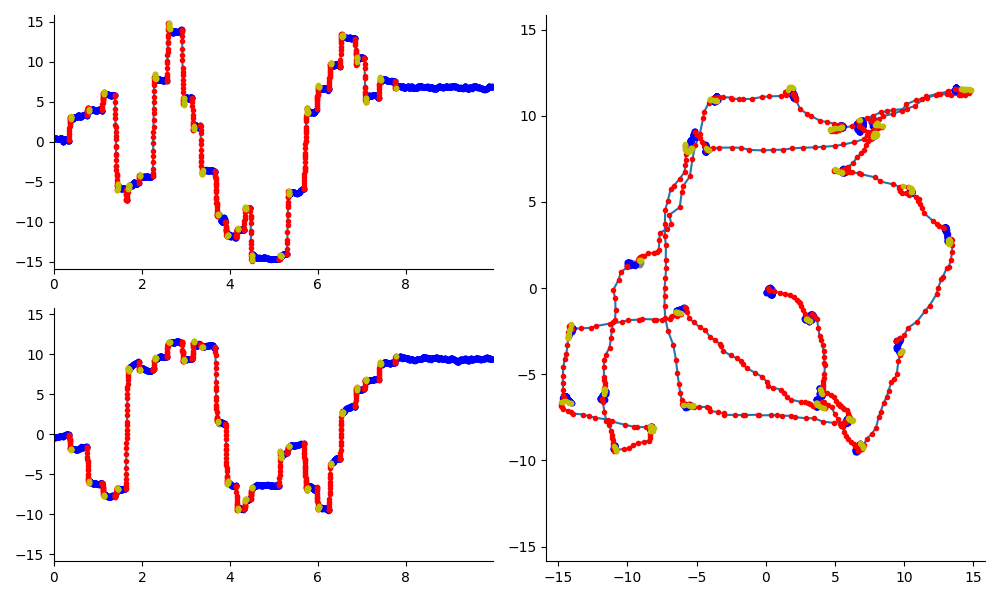
\includegraphics[width=0.7\linewidth]
    {TH34_img_Europe_labelled_MN}
    \label{fig:lund2013}
    \caption{The two graphs on the left show the x and y coordinates of the gaze position in degrees over time in seconds. The graph on the right resembles the gaze position in the x-y-plane. The red dots represent fixations, the blue dots represent saccades and the green dots represent post saccadic oscillations.}
\end{figure*}

\subsection{Conversion script}
In order to allow maximum flexibility for future users of gazeNet a script is provided which converts .csv/.tsv eye-tracking data files into the proprietary datatype ETData used by gazeNet. The script works on both Windows and UNIX-like operating systems thanks to pathlib which handles path and file names. Even though slight modification may be necessary, the given script should provide a useful template for the preparation of similarly formatted gaze recordings.

In this particular case the file to be converted stems from an eye tracker made by Tobii. Each sample of the recording is stored in a separate row. The gaze coordinates are stored in the columns "Gaze point X" and "Gaze point Y" in cartesian form as pixels and can therefore be used as they are. The custom datatype requires information about the geometry of the test setup in order to internally convert the cartesian coordinates to polar coordinates. As of now these parameters are hardcoded in the script. Finally invalid samples are filtered.

\subsection{Validation of gazeNet 0.1}
In \citet{zemblys2018gazeNet} the authors rely heavily on the lund2013-image-test dataset in the development of their framework, which makes it a good choice for validation of the updated gazeNet. Figure \ref{fig:lund2013} shows the output of gazeNet 0.1 on the lund2013-image-test dataset. The results are comparable to the results presented in \citet{zemblys2018gazeNet}. 

The working of the conversion script has been shown on a recording of a participant looking at randomly appearing crosses on a screen. Figure \ref{fig:kreuze} shows the output of gazeNet 0.1 on the recording. The results are comparable to the results presented in \citet{zemblys2018gazeNet}.

\begin{figure}
    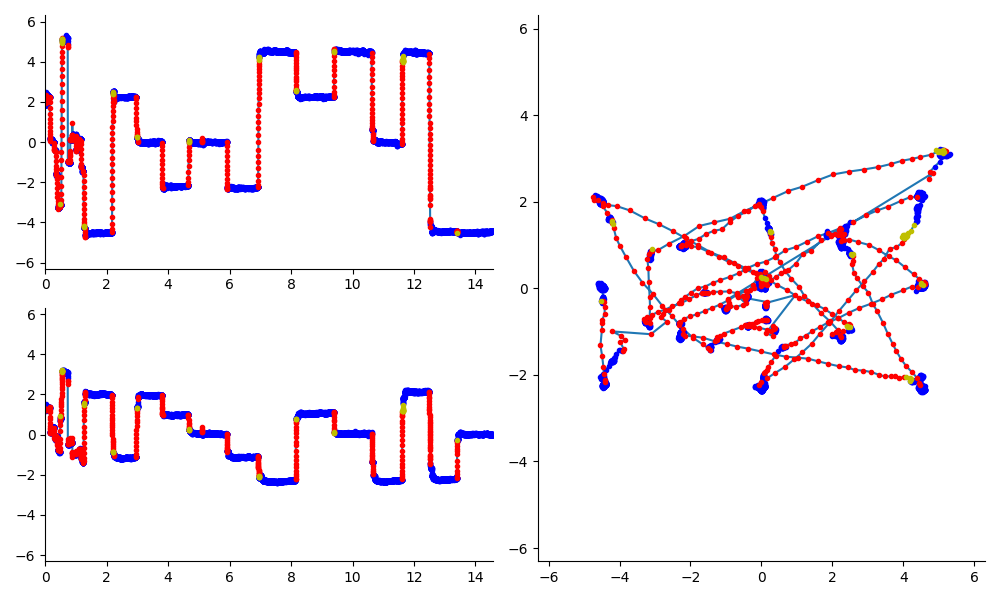
\includegraphics[width=\linewidth]{Kreuze_Random Recording1_short}
    \label{fig:kreuze}
    \caption{The two graphs on the left show the x and y coordinates of the gaze position in degrees over time in seconds. The graph on the right resembles the gaze position in the x-y-plane. The red dots represent fixations, the blue dots represent saccades and the green dots represent post saccadic oscillations. It should be noted that the first two seconds of the recording contain the calibration points of the eye tracker. The calibration process contains events on which gazeNet is not trained. Therefore the labelling is insignificant.}
\end{figure}

\section{Future work}
Even though the update to gazeNet 0.1 has increased useability there is still a lot of work that can be done in order to make this tool even more accessible. Especially considering the framework, as it is now, still only being a proof-of-concept already being so valuable, the potential cannot be underestimated. Areas of further development should either improve gazeNet in functionality or in ease of use.

\subsection{Functionality}
At the time of writing the pretrained neural network can only label fixations, saccades and post saccadic oscillations. Logically it would make sense to expand the types of events such as continuos pursuit that can be detected. One way to realize this would be to train a new network including data containing also said event types. The challenge hereby, apart from ``obtaining reliably coded eye-tracking data'' \citet{zemblys2018gazeNet}, lies in training an algorithm, that ``can perform as well as human expert coders'' \citet{zemblys2018gazeNet}. It has yet to be seen if adding even only one new event type to be recognized has a negative impact on accuracy. If this should be the case, a possible solution might be to change the architecture of the neural network.

\subsection{Ease of use}
The addition of the conversion script has already opened up the possibility of using gazeNet with data from other eye trackers than the one used by the authors. However, at this point it is still necessary to clone the repository and work with the code more or less directly i.e. installing dependencies. A more user-friendly approach would be to provide a package that can be installed via pip. The user would then only have to import the package and call the appropriate functions.

Taking this thought even further, the user could be provided with a graphical user interface (GUI) to interact with gazeNet. This would allow the user to work with gazeNet without having to write a single line of code. The GUI could be implemented as a jupyter notebook, which would allow the user to work with gazeNet on any device with a web browser. The user would then only have to upload the data to be analyzed, define the geometry of the eye-tracking setup and download the results.

\bibliographystyle{plainnat}
\bibliography{gazeNet.bib}
\end{document}